\chapter{Research Design}
\label{resdes}
\begin{comment}

\end{comment}

\begin{figure}[h]
	\centering
	\captionsetup{justification=centering}
\scalebox{.40}{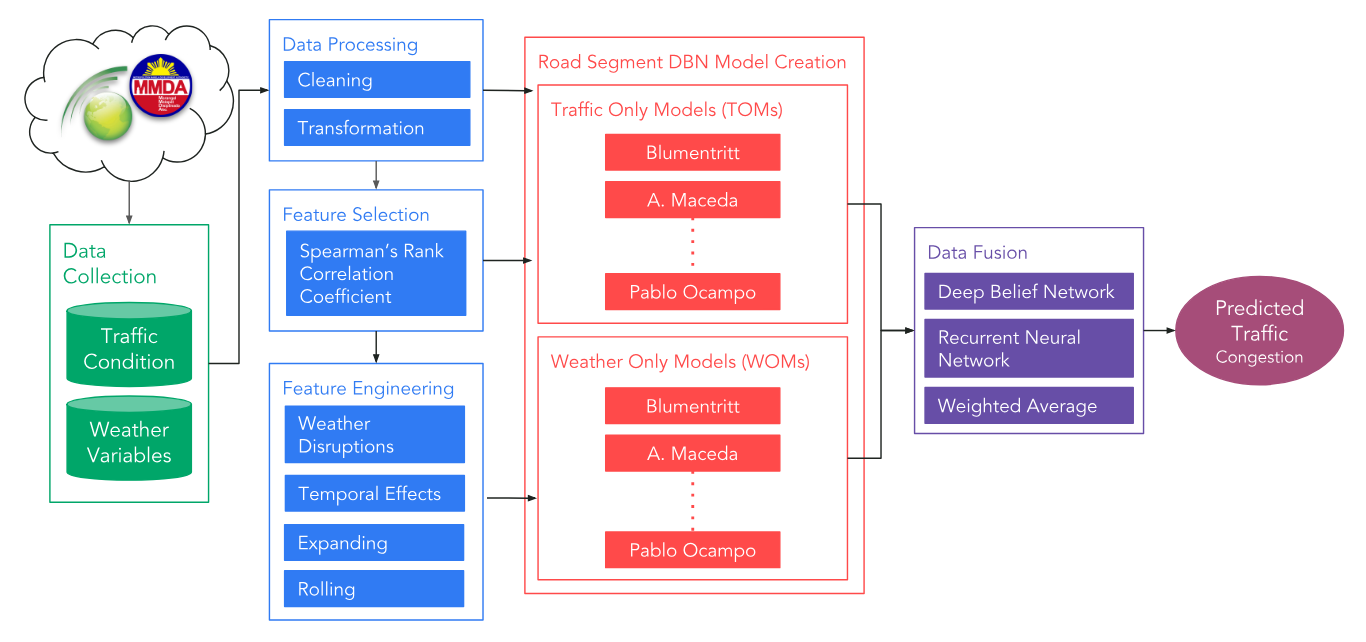
\includegraphics{THESIS_ResearchDesignFinal.png}}
	\caption{Research Framework}
	\label{fig:framework}
\end{figure}




Figure \ref{fig:framework} illustrates the whole framework for the research. First, this research collected historical traffic condition from MMDA and historical weather variables from WWO. These raw data were cleaned and re-sampled to match the time intervals of the data using linear interpolation and was transformed to their normalized values. The data was explored and analyzed to identify seasonality and trends present for both traffic and weather. Analyses and insights collected were used to select and engineer features to use in the model to predict traffic. These features include rolling and expanding window features, which are in-depth statistical features of traffic such as the mean, minimum, and maximum values of past traffic of a certain time period.

The final variables and engineered features were fed into the Traffic-Only Models (TOM) and Weather-Only Models (WOM), which were developed in DBN, for the 14 road segments in Manila for both wet and dry season. Additionally, analyses were evaluated through the training of the models. Two different fusion levels were tested in this model, specifically at the feature level and at the decision level. For the decision level, three fusion techniques were tested, particularly DBN, RNN, and WA. The model was evaluated using RMSE and MAE. The model’s sensitivity was also explored to analyze the relevance of input variables. 

\section{Data Collection}
\label{rd_datacollection}
There were two public datasets collected: one for traffic and one for weather. The traffic dataset was obtained from Metro Manila Development Authority (MMDA) traffic monitoring system, while the weather dataset was collected from World Weather Online (WWO). Both datasets were collected from January 2015 to December 2015.

\subsection{Traffic Dataset}
There were two limitations found from the traffic dataset. First is that the traffic conditions were only represented as \textit{light} (L), \textit{moderately light} (ML), \textit{moderate} (M), \textit{moderately heavy} (MH), and \textit{heavy} (H). Since this dataset only had five values to classify the traffic condition in a particular road segment, this might cause underfitting in our model since it was used as input for a regression problem. Moreover, it could also contribute to poor correlation as these five values were correlated with continuous weather variable values. To have the traffic conditions be continuous values, they were converted to their equivalent estimated traffic speed provided by the MMDA (see Table \ref{table_traffic_condition}). These speeds are further converted to congestion levels, represented as their reciprocal so that the data would be easier to interpret such that higher value means higher congestion level.

\begin{table}[h]
\centering
\caption{Traffic speed equivalent of traffic conditions}
\label{table_traffic_condition}
\begin{tabular}{|l|r|}
\hline
\textbf{Traffic Condition} & \multicolumn{1}{l|}{\textbf{Equivalent Speed (kph)}} \\ \hline
Light (L) & 36 - 60 \\ \hline
Moderately Light (ML) & 31 - 35 \\ \hline
Moderate (M) & 16 - 30 \\ \hline
Moderately Heavy (MH) & 11 - 15 \\ \hline
Heavy (H) & 0 - 10 \\ \hline
\end{tabular}
\end{table}

Another limitation was that the traffic dataset contains missing records. Out of 935,200 records, there were 93 rows wherein the traffic condition of that road segment in that particular time interval was not recorded as indicated by \textit{none} (N) condition. Furthermore, having only 935,200 records from a sample from 2015, having a 15-minute interval for 14 road segments, meant that 45,920 records were missing as well. This implied that inconsistencies may occur as the missing data would need to be filled to make the data continuous. To do this, those missing values were replaced through linear interpolation. 

Apart from the limitations, there were other factors considered in this study. Since this study is only concerned road segments from Manila, only the road segments under it were used. As a result, 14 out of 142 road segments were only considered: 7 from Roxas Boulevard and 7 from España.

\subsection{Weather Data}
The collected weather dataset from WWO featured a complete hourly reading of the weather variables for Manila. One downside of this dataset, however, was that the weather data generalizes the weather for the whole city. This implied inconsistencies when correlating the traffic condition to the weather variables as the weather at one road is not the same as the weather of another, despite being in the same city.

Additionally, the hourly weather dataset needed to be matched with the 15-minute interval of the traffic dataset. This was done by resampling and linear interpolating the dataset to have a 15-minute time interval.

\section{Exploratory Data Analysis}
To be able to extract the relationship between these two independent datasets, it is important to understand the underlying pattern of each dataset and its effect on one another. In this study, analysis was  done in three steps. First, patterns of traffic and weather are explored as independent entities. These patterns include seasonality and trends of each variable, and disruptions present for each variable. Second, these patterns are compared to identify the relationship between the two entities. Third, once these patterns are bridged, instances of weather disruption to traffic are derived by associating the weather variables that may be a contributing factor to traffic.

\subsection{Seasonality Analysis}
Seasonality refers to a predictable pattern of a time series data that regularly repeats after a number of intervals. To identify the short-term seasonality of weather variables, the similarity between an observation and time lags between them were analyzed through autocorrelation. \textit{Lags} refer to the time delay of one observation on another. For instance, the delay between the temperature observations at June 18 and June 19 is indicated by a one-day lag.

\subsubsection{Weather Seasonality}
%Seasonality
Assessing the seasonality of weather variables is necessary to identify the span of the trend of a specific weather variable. Observably, one weather variables that do have a daily pattern is temperature. Its pattern starts by rising in the morning, peaking in the afternoon, then starts falling in the evening. There are also weather variables, on the other hand, that does not have an observable pattern. One example of this is precipitation. Unlike temperature that has an observable pattern per day, the occurrence of precipitation is situational. In this part of analysis, some weather variables would be identified to have a daily pattern and also the ones with no pattern at all. 

%Trend
Aside from the seasonality of each weather variable, their trends are also explored, based on the identified seasonality time spans. These trends were then compared to the short-term seasonality to determine the similarities with each other. For instance, the temperature on one observation was compared to its previous day, as well as the precipitation on one observation and its previous day.

\subsubsection{Weather Disruptions}
Assessing the effect of a disruption of one weather variable to another weather variable was also explored. After analyzing the seasonality of weather, its normal trend is defined. Any other patterns that are significantly different from the defined normal trend of any weather variable were explored and compared with other aligned weather variables.

\subsubsection{Traffic Seasonality}
On an average day, traffic could be linked with the people's daily transportation demand. One example of these is the daily commute of people, attributed to their organizational duties (i.e. 9 to 5 jobs) and academical duties. Built upon these expected demands, the daily seasonality of traffic has been established, following the concept of peak hour. Peak hour refers to the busiest hour where traffic is expected to rapidly rise. In the case of Metro Manila, peak hours are expected to occur from 7 AM to 10 AM, when people leave their home to go to their respective organizations, and 4 PM to 7 PM, when they depart their organizations and return home (Regidor, 2013).

However, knowing that there are other contributing factors to traffic, its pattern is inconsistent despite its people’s daily commute schedule remains constant as the years go by. Given this problem, it is significant to identify the more accurate estimate of the seasonality of traffic, considering that these contributing factors are already embedded in the day-to-day traffic. These could be done by analyzing a road segment, as an individual point-to-point segment, and analyzing a road segment, as a part of the whole road, taking into account its connected roads.

\subsubsection{Traffic Disruptions}
As traffic seasonality was explored, traffic patterns that do not follow the defined pattern is explored. Disruptions in the patterns of traffic is compared with the explored disruption in weather to derive an analysis whether the disruptions of traffic and weather are connected.

\section{Correlation Analysis}
The relationship of weather and traffic is then explored through correlation analysis, using Spearman’s  correlation coefficient. In this analysis, correlations between weather variables, connected roads, and engineered traffic features with traffic were explored in order to have a better understanding of the effect of weather to traffic, especially in time periods where weather is most expected to disrupt traffic such as periods typhoons are present. Relationships derived from the correlation were verified through comparative analysis between the defined weather and traffic patterns.

First, the relationship of each weather variable to one another was explored in order to extract which weather variables are significant with respect to traffic condition. Significant weather variables that are both highly correlation with another variable, but less correlated with traffic than the other variable is removed to reduce redundancy. Then, the relationship between connected roads was explored. In this analysis, the intensity of one road segment and its effect to the connected road segment was analyzed through correlation. The correlation growth from the first road segment, to the nth connected road segment was also analyzed. Lastly, the relationship between the engineered traffic features to the current traffic feature. Before exploring this relationship, traffic features were engineered from the current traffic feature in order to give information of the immediate past traffic, and its relationship with the current traffic. These engineered traffic features include rolling and expanding window features, statistical description of past time period such as the mean traffic two (2) weeks ago, and flags for significant traffic patterns such as the work day and peak hours. Exploring the relationship between these engineered traffic features with the current traffic feature also give a better representation of the effect of disruptions present in the immediate past to the current traffic.

As mentioned, rolling and expanding window features were engineered to represent the immediate past traffic. Rolling and expanding traffic features were generated for window sizes \textit{4, 8, 24, 48}, and \textit{96}, with each window representing a 15-minute time interval. Thereby, the generated window sizes translates to \textit{1, 2, 6, 12}, and \textit{24}-hours time interval. The statistical features such as the mean, minimum, and maximum for both rolling and expanding windows were generated to describe the immediate past traffic conditions given a specific window size.



%TRAFFIC MODEL CREATION
\section{Model Implementation}
Features were engineered in order to represent the immediate past traffic, and other trends and patterns of traffic. Additionally, weather features were selected through correlation analysis. These features are as follows:

\begin{enumerate}
\item Temporal Information of the respective traffic record represented as Month, Day, Hour, Minute, Day of Week,
\item Traffic a Day before represented as L, ML, M, MH, H
\item Traffic 6 weeks ago represented as L, ML, M, MH, H
\item Current Traffic represented as L, ML, M, MH, H
\item Rolling and Expanding Traffic Features (mean, max, and minimum) for windows 4, 8, 24, 48, and 96 represented as L, ML, M, MH, H,
\item Weather Variables (wind speed, wind gust, temperature, humidity, dew point, precipitation, visibility, pressure, cloud cover, heat index, and feels-like) represented in their respective measurements
\end{enumerate}

A model implemented using Deep Belief Network (DBN) used these features that represent the past traffic to predict the current traffic condition intensity.

\subsection{Prediction Models}
According to the framework in \ref{fig:framework}, two models were implemented using Deep Belief Network (DBN): the Traffic-Only Model (TOM) and the Weather-Only Model (WOM). The TOM considers historical traffic condition intensity to predict traffic, while the WOM only considers historical weather variables to predict traffic. In this study, these DBN models were implemented with the open source machine learning framework in Python, \textit{tensorflow}. For the TOM, there are two hidden layers with 14 and 375 units respectively. The TOM was trained with 11 epochs during the pre-training phase, and 80 epochs during the fine-tuning phase. For the WOM, there are 3 hidden layers with 14, 85, and 170 units respectively. The WOM was trained with 5 epochs during the pre-training phase, and 88 epoch during the fine-tuning phase. The learning rate for both models DBN is 0.01 and and RBM is 0.0. The activation function for both models is the $relu$ function.

DBNs are made up of stacks of Restricted Boltzmann Machines. The training for DBN consists of two phases: pre-training and fine-tuning. In pre-training, each RBM is trained individually, and weights and biases of layers are fixed. In fine-tuning, the weights and biases of the whole network are updated via back propagation using labeled input data.

Figure \ref{fig:dbntraining} shows the process of how the TOM and the WOM using DBN was trained for prediction. The training process consists of three phases. In the first phase, the stacks of RBM (sRBM) within the network are trained individually. At the end of this phase, the weights and biases of the whole DBN are initialized. In the second phase, the DBN fine tunes the initialized weights and biases using backpropagation algorithm. The network after stage 2 is the trained and enhanced DBN. In the third phase, the network predicts the future traffic condition using a testing dataset.

\begin{figure}[h]
	\centering
	\captionsetup{justification=centering}
	\scalebox{.8}{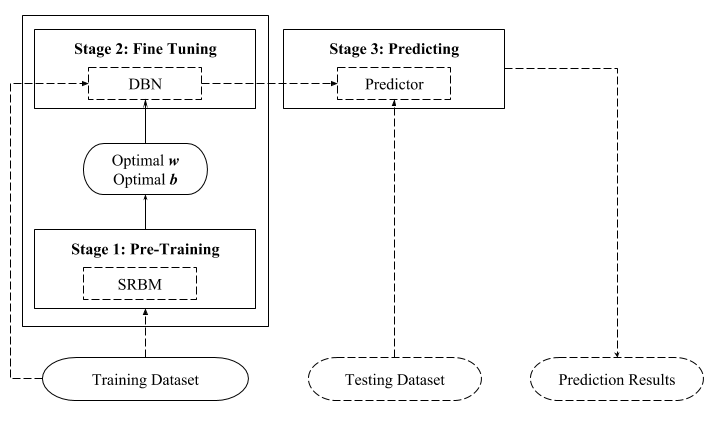
\includegraphics{dbntraining.png}}
	\caption{Structure of DBN Training Process}
	\label{fig:dbntraining}
\end{figure}

For the pre-training phase, the sRBM performs a number of forward and backward passes until the reconstructed data is close to the original input. The process of backward and forward passes is performed using the equations \ref{eq:4} and \ref{eq:5} to compute for the conditional probability of the hidden unit $h_j$ and visible unit $v_i$, respectively.

%Fine Tuning
For the fine-tuning phase, the loss function and activation function is defined.
The loss function for the softmax layer to improve the learning rate uses the cross-entropy equation between the visible and hidden units. The cross-entropy function is defined as
\begin{equation}
C = -\frac{1}{n}\sum_x [y ln a + (1 - y) ln (1-a)]
\end{equation}
\noindent where $n$ is the size of the training data, $x$ is the training input, $y$ is the desired output, and $a$ is the unit’s output.
For the activation function in the fine-tuning phase, the rectifier function was used for its nonlinearity activation capability. The rectifier function is defined as
\begin{equation}
f(x) = x^+ = max(0, x)
\end{equation}


\subsection{Data Fusion Model}
This study evaluated two fusion approaches: Feature In-Decision Out (FEI-DEO) and Decision In-Decision-Out (DEI-DEO). In the FEI-DEO approach, traffic and weather features are fused in one dataset first before being used by the model to predict traffic. The DEI-DEO approach, meanwhile, predicts traffic through TOM and WOM, and fuses the prediction of both models into one final prediction. DBN is used in the FEI-DEO approach, while three algorithms are tested in the DEI-DEO approach which are Weighted Average (WA), Recurrent Neural Network (RNN) and DBN.


%WEIGHTED AVERAGE
\subsubsection{Weighted Average}
The weighted average data fusion method used the predicted traffic from TOM and WOM. Both predictions was multiplied with its corresponding weight. Each weight was assigned based on the importance of the variable considered while keeping in mind the sum of the weights should be equal to 1. Then, the mean of the weighted predictions of both TOM and WOM will be calculated. The result will be the fused final traffic prediction.


%NEURAL NETWORK
\subsubsection{Neural Network}
The fusion model was also developed in two neural networks: Recurrent Neural Network (RNN) and Deep Belief Network (DBN) in evaluating DEI-DEO fusion approach. Only DBN was implemented in evaluating FEI-DEO approach.

In FEI-DEO, the traffic congestion intensity and weather variables were fused into one dataset before feeding it into the prediction model. The network will be trained to predict the traffic condition based from both traffic and weather in one model for the current time period $t$. The training of the network will continuously adjust weights and biases from comparing the generated output with the actual traffic condition.

The DBN for FEI-DEO fusion have 1 input layer, 3 hidden layers, and 1 output layer. There are 5 epochs for the pre-training phase, and 150 epochs for the fine-tuning phase. The learning rate for both DBN and RBM is 0.01.

In DEI-DEO, the traffic congestion intensity was predicted first with two prediction models, TOM and WOM. The prediction by these two prediction models was used into another model that will fuse the two predictions into one improved final prediction. The network will be trained to predict the traffic congestion intensity for the current time period $t$ through backpropagation by comparing the generated traffic condition prediction to the expected prediction, and adjusting the weights and biases of units and layers to fuse the two decisions to arrive to a prediction close to the expected. The input layer will have the predicted traffic condition of TOM and WOM.

The RNN for DEI-DEO fusion have only have 1 input layer, 1 hidden layer, and 1 output layer. The number of units for the hidden layer of the RNN will be determined through trial and testing starting from 5 to 100 units.

The DBN for DEI-DEO fusion will only have 1 input layer, 3 hidden layers, and 1 output layer. The DBN for the DEI-DEO fusion will be similar with the TOM and WOM in terms of it’s hidden layer structure, and epochs. However, instead of historical traffic and weather data as its input, predictions made by TOM and WOM is used and fused into one final prediction.

%TRAINING
\section{Training}
The collected dataset for traffic and weather was divided into two subsets; wet and dry season. The wet season dataset consists of data from the months of May to October 2015, while the dry season dataset consists of data from the months of November to April 2015. The models was tested on these datasets to evaluate the inclusion of weather variables.

Datasets was split into training and testing datasets. The training dataset was used during the pre-training and fine-tuning of the model. In the fine-tuning phase of the training of the model, the training dataset was labeled with the expected output so as to verify and adjust the weights and biases back from the pre-training. The label consists of the expected traffic condition given the input data. All data fed into the network are already be normalized.

The training dataset for both prediction models TOM and WOM consists of data from the months of May to August was used for evaluating wet season, and months of January to April was used for evaluating dry season. In turn, the testing dataset made use of the remaining months of the season: September to October for the wet season, and November to December for the dry season.

%[Training Data of TOM]
The training dataset for the Traffic-Only Model consists of the following information in a 15-minute time interval:

\begin{enumerate}
\item Temporal information of the respective time period (i.e. month, hour, minute, day, and day of week);
\item Traffic condition intensity a day before the respective traffic;
\item Flags on working day and peak hour of the respective time period;
\item Rolling and expanding window features (which consist of the minimum, maximum, and mean for each window) for the immediate past traffic of the respective traffic; and
\item Average traffic 2 weeks before the respective traffic.
\end{enumerate}

In further experiments, the inclusion of the information regarding working days, peak hours, and immediate past traffic was compared and evaluated. The label for the training dataset consists of actal the 15-minute time interval of the traffic condition intensity of the respective time of the bound of the road segment to be predicted. For visualization purposes, the input including the labels is illustrated in Figure \ref{fig:TOM_TrainingTestingInput}


\begin{figure}
\centering
\captionsetup{justification=centering}
\scalebox{.70}{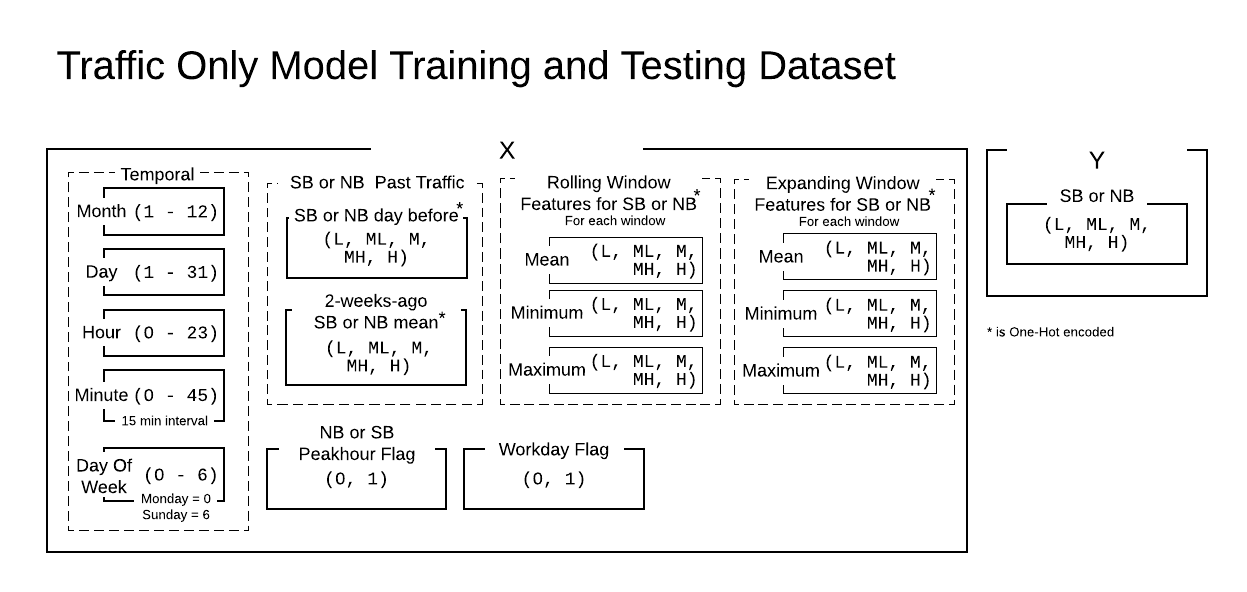
\includegraphics{TOM_TrainingTestingInput.png}}
\caption{A summary on the contents of the Traffic Only Model Training and Testing Dataset}
\label{fig:TOM_TrainingTestingInput}
\end{figure}


%[Training Data of WOM]
The training dataset for the Weather-Only Model consists of the following information in a 15-minute time interval:

\begin{enumerate}
\item Temporal Information of the respective time period (i.e. month, hour, minute, day, and day of week); and
\item Current weather variables (e.g. temperature, precipitation, wind speed, etc.) of the respective time period.
\end{enumerate}

In further experiments, different combinations of weather variables is compared and evaluated. The label for the training dataset consists of the actual 15-minute time interval of the traffic condition intensity of the respective time of the bound of the road segment to be predicted.

%[Training Data of DF Fusion Model]
For the FEI-DEO model, the training dataset consists of merged training dataset used in the TOM and the WOM. The months for the training and testing datasets for this fusion model is also the same.

For the DEI-DEO model, the training dataset consists of the predicted traffic generated by TOM and WOM. The months for the training consists of the months of May to September for the wet season, and January to April and November to December for the dry season. The testing dataset consists of the predicted traffic for the month of October and December. The label for the training dataset will consist of the 15-minute time interval of the actual traffic condition intensity of the respective time of the bound of the road segment to be predicted.


\section{Evaluation}
%[Comparing of Performances]
The performance of the all models and algorithms (DBN, RNN, and WA) was evaluated using RMSE and MAPE. The performance of the fusion model fusing in the feature level (FEI-DEO) and in the decision level (DEI-DEO) was first evaluated. In evaluating DEI-DEO, the performance of the TOM and the WOM models were initially evaluated before the fusion model/s. The performance of the TOM and the WOM with different feature combinations are compared with each other to see which input variables are needed in predicting the traffic condition intensity in current time period $t$. Then, three fusion techniques, namely WA, RNN and DBN, were compared and evaluated to see the accuracy of the final prediction. Additionally, the performance of the TOM and the final prediction of the DEI-DEO fusion model was evaluated to see relevance of the inclusion of weather variables as a factor in predicting traffic.

The model’s sensitivity was also explored to analyze the relevance of input variables. Sensitivity analysis is also performed to achieve higher accuracy through calibration of hyper parameters. Specifically, the sensitivity for the models TOM, WOM and DEI-DEO fusion center in DBN were evaluated. In evaluating the sensitivity for TOM and WOM, different combinations of input variables were evaluated to see how much the inclusion and removal of a variable affects the final prediction. The parameters of the network was also experimented with, specifically the number of hidden layers and its units, the number of epochs for pre-training, the fine-tuning, and the batch size.





